\section{Engineering Challenges}
Research challenges such as static analysis of exit points and veritesting in a multi-threaded context need to be solved for integrating veritesting with any bytecode-level symbolic execution engine.
%
Symbolic PathFinder is a popular Java bytecode-level symbolic execution tool.
%
It has been used to find bugs in flight software~\cite{pasareanu2008}, to test large web applications~\cite{fujitsu}, and for testing Android apps~\cite{android_spf}.
%
It has also been extended for parallel symbolic execution~\cite{parallel}, and for load testing~\cite{load_testing_spf}.
%Talk about the engineering challenges we face when implementing veritesting with Symbolic PathFinder
%
Given the large and diverse set of applications that stand to benefit from integrating veritesting with SPF, we discuss here the engineering challenges expected with such an integration.

\subsection{Shared Expressions}
%Sharing implementation needs to be fixed. Show this using the TestSharing example
Veritesting causes regions of code to be executed using static symbolic execution.
%
Symbolic formulas representing the static symbolic execution are then gathered at the exit points of the region and added to the path expression and symbolic store of dynamic symbolic execution.
%
This causes large disjunctive formulas to be substituted and reused multiple times, necessitating the use of techniques like hash consing~\cite{hashconsing}, or its variants such as maximally-shared graphs~\cite{babic}, or using expression caching~\cite{green}.
%
To evaluate reuse of structurally equivalent expressions in SPF, consider the code shown in Listing~\ref{lst:sharing}.
%
\lstinputlisting[caption={An example with an increasing formula size with every loop iteration},
label={lst:sharing}]{code_samples/TestSharing.java}
%
The function \textit{testSharing} adds the value of \textit{x} to itself in every loop iteration on line 3 of Listing~\ref{lst:sharing}.
%
The number of loop iterations is controlled by a user-supplied value for \textit{bound}.
%
On line 4, the code branches on the value of the value of \textit{x}.
%
We symbolically executed the \textit{testSharing} method with \textit{x} set to be symbolic and \textit{bound} set to be a concrete value.
%
We set the minimum and maximum symbolic integer values to be -100 and 100 respectively.
%
We increased the value of \textit{bound} from 1 to 29 and recorded the time taken for complete path coverage.
%
Figure~\ref{fig:sharing_time} shows the trend seen for increasing values of \textit{bound}.
%
Figure~\ref{fig:sharing_time} shows that the running time remains constant until the value for \textit{bound} is 18, and then starts to rise exponentially. \mike{These figures are {\em way} too large.  They could be compressed both vertically and horizontally to fit into one column while still telling the story}
%
We also recorded the maximum memory usage reported by SPF for increasing values of \textit{bound}, and present our observation in Figure~\ref{fig:sharing_mem}.

\begin{figure}%
    \centering
    \subfloat[Time required for covering paths in Listing~\ref{lst:sharing}]{{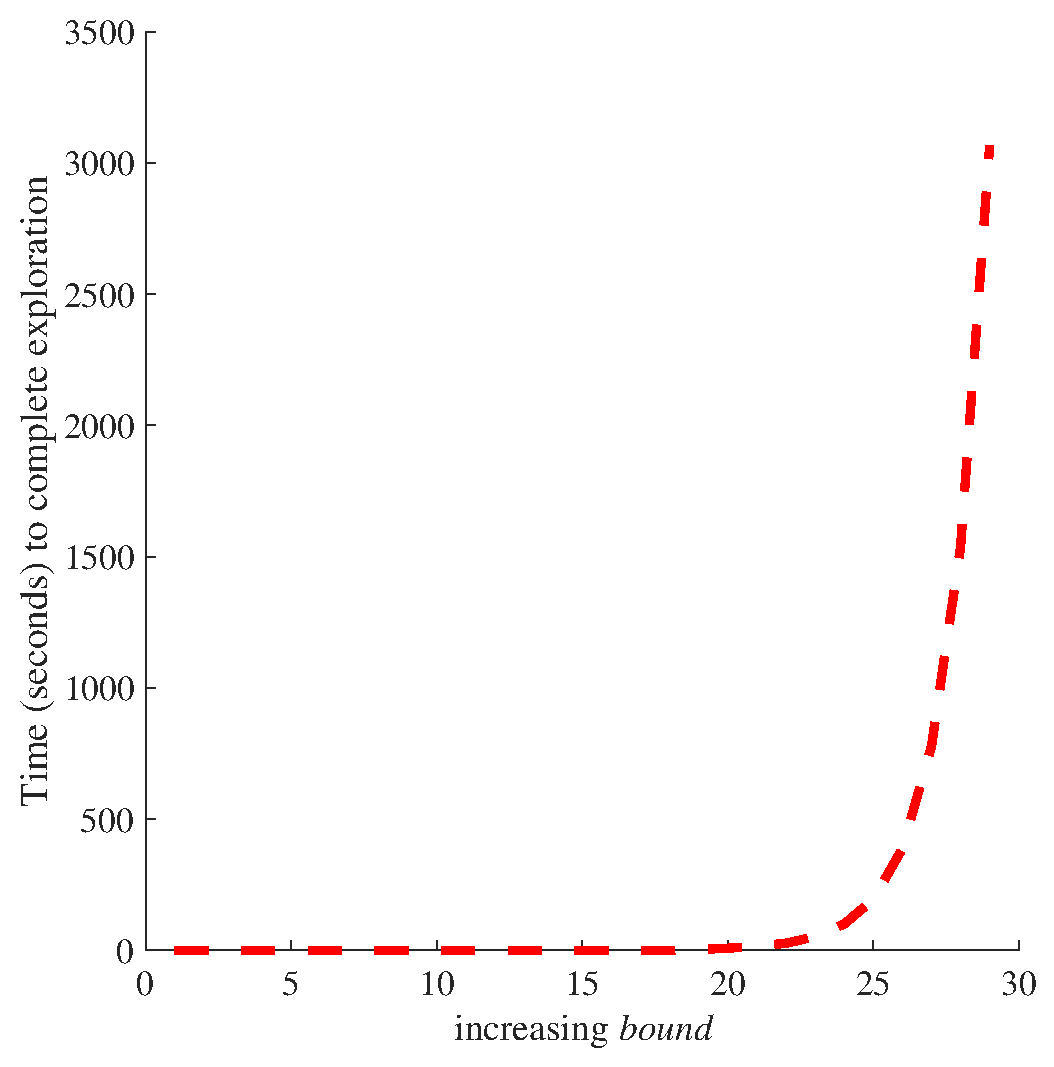
\includegraphics[width=0.4\columnwidth]{figures/sharing_time} }\label{fig:sharing_time}}%
    \qquad
    \subfloat[Maximum memory usage of SPF for covering paths in Listing~\ref{lst:sharing}]{{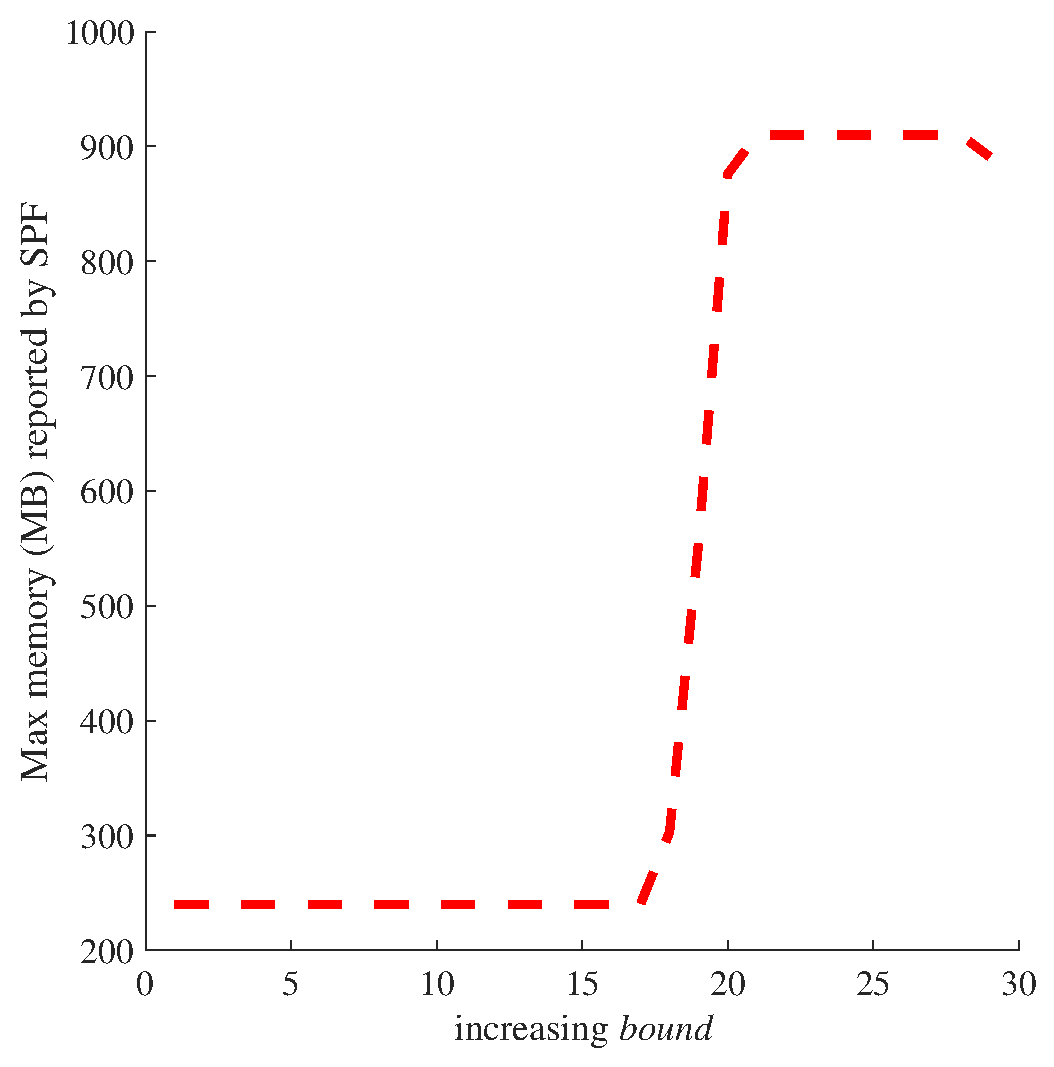
\includegraphics[width=0.4\columnwidth]{figures/sharing_mem} }\label{fig:sharing_mem}}%
    \caption{Time and memory usage of Listing~\ref{lst:sharing} when increasing \textit{bound}}%
    \label{fig:sharing}%
\end{figure}
%
We observe that at a value of 17 for \textit{bound}, the memory usage starts to rise from 240 MB and has reached 910 MB when \textit{bound} equals 21.
%
We also observed that the number of expression objects undergoes a linear increase with the value of \textit{bound}.
%
These three observations lead us to the hypothesis that while SPF does share expression objects internally, the traversal of such expressions breaks the sharing and causes an increase in time and memory.\mike{The time increase is (I suspect) due to garbage collection once the maximum memory threshold is reached. This may or may not be worth mentioning.}
%
Integrating veritesting with SPF to make it scale to industrial-sized code requires resolving such engineering issues.
%
\subsection{Complex Expressions}
%Engineering issue \#2: Need to have complex expressions, talk about how Comparators cannot be used anywhere below the top-level operator
SPF creates conjunctions of expressions and adds them to its path expression.
%
The expression being added to its \textit{PathCondition} is allowed to have a \textit{Comparator}~(a comparison operator such as !=) as the top-level operator, but comparison operators are not allowed in sub-expressions.
%
But, symbolic formulas derived from static symbolic execution of regions does not guarantee that such an invariant would always hold for formulas.
%
This design choice prevents symbolic formulas derived from static symbolic execution from being added to SPF\rq s path expression.
%
SPF\rq s design needs to be changed to allow comparison operators in sub-expressions.
%
But, because SPF has different classes for different expression types~(\textit{IntegerExpressions}, \textit{RealExpression}), this design change has to be made once for each expression type.
%
Thus, integrating veritesting presents a design challenge to allow complex expressions in SPF.
%
% \subsection{Intermediate variables}
% %Engineering issue \#3: Nice to introduce intermediate variables
% %
% During veritesting, symbolic formulas derived from static symbolic execution of a region may involve conditional write operations into other variables.
% %
% It is convenient to have intermediate variables~(one per variable written to in the region) which capture such conditional write expressions during the static symbolic execution.
% %
% Later, at an exit point, the intermediate variables can be written into the original variables written to in the region.
% %
% This allows sub-expressions to be shared, and even simplified, without affecting the original variables from the Java bytecode.
% %
% Smaller formulas written into the region\rq s output variables also makes it easier to debug veritesting of regions.
% %
% However, creation of such intermediate variables presents a design challenge in SPF.
% %
% SPF stores and propagates symbolic information through attribute objects.
% %
% This, in turn, creates an invariant that every symbolic variable in the path expression needs to be mapped to an attribute object.
